% Graph: Análise do tempo de geração por chave com desvio padrão no Experimento Gamma
\begin{figure}[H]
	\centering
	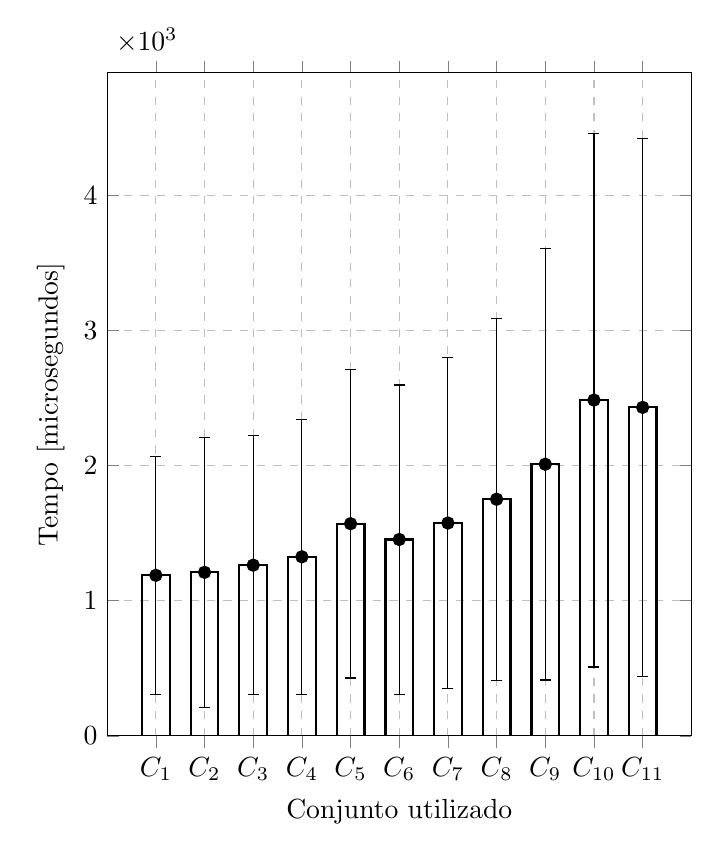
\begin{tikzpicture}
		\begin{axis}[
			% title={Análise do tempo de geração com desvio padrão},
			symbolic x coords={$C_1$, $C_2$, $C_3$, $C_4$, $C_5$, $C_6$, $C_7$, $C_8$, $C_9$, $C_{10}$, $C_{11}$},
			xtick={$C_1$, $C_2$, $C_3$, $C_4$, $C_5$, $C_6$, $C_7$, $C_8$, $C_9$, $C_{10}$, $C_{11}$},
			ylabel={Tempo [microsegundos]},
			xlabel={Conjunto utilizado},
			ybar,
			ymin=0,
			bar width=10pt,
			ymajorgrids=true,
			xmajorgrids=true,
			grid style=dashed,
			height=10cm,
			width=9cm,
			tick scale binop=\times,
			scaled y ticks=base 10:-3,
		]
		 
		\addplot[color=black, solid, thick, mark=*] plot[error bars/.cd, y dir=both, y explicit]
			coordinates {
				($C_1$,1188) +- (1496.8,879.2)
				($C_2$,1210) +- (1419.9,1000.1)
				($C_3$,1263) +- (1568.2,957.8)
				($C_4$,1325) +- (1631.8,1018.2)
				($C_5$,1570) +- (1920.4,1142.1)
				($C_6$,1453) +- (1762,1144)
				($C_7$,1575) +- (1925.4,1224.6)
				($C_8$,1751) +- (2162,1340)
				($C_9$,2010) +- (2423,1597)
				($C_{10}$,2485) +- (2991.7,1975.3)
				($C_{11}$,2431) +- (2853.9,1990.1)
			}; %\legend{\Bytes}

		\end{axis}
	\end{tikzpicture}
	\caption{Análise do tempo de geração com desvio padrão.}
	\label{graph:timeResultsGamma}
\end{figure}